\chapter{基于反事实样本生成的视觉问答方法}

随着计算机视觉和自然语言处理等技术的发展,视觉问答技术在过去的十年间取得了长足的进步。然而,目前的视觉问答模型仍然过于依赖问题与答案之间的联系(即文本偏置)。为了缓解这一问题,近期的一些视觉问答模型开始通过引入一个辅助网络来约束视觉问答模型的训练。这种复合模型在标准视觉问答数据集VQA-CP上取得了当时最好的实验性能。但是,由于这类复合模型设计的复杂性,它们往往难以满足一个理想视觉问答模型应该具备的两个特性:(1)视觉可解释性(visual-explainable ability):当预测答案时,模型应该基于正确的视觉图像区域。(2)问题敏感性(question-sensitive ability):当改变问题时,模型应该能够感知问题的变化,并对预测结果做出相应的调整。因此,在本章,我们提出了一种通用的反事实样本生成机制(Counterfactual Samples Synthesizing, CSS)。CSS机制通过遮盖图像中的重要区域或问题中的重要单词来合成新的反事实训练样本,并且对这些反事实样本赋予不同的标准答案。通过使用原始训练样本和新合成的反事实样本一起对模型进行训练,能够迫使模型关注被遮盖的重要区域和单词,进而提升模型的视觉可解释性和问题敏感性。另一方面,随着模型的视觉可解释性和问题敏感性得到提升,模型更减少对文本偏置的依赖,进一步提升模型视觉问答性能。在视觉问答数据集VQA-CP中,我们通过大量的对比实验验证了CSS机制的有效性。值得注意的是,当对视觉问答模型LMH~\cite{clark2019don}使用CSS机制进行训练后,模型在数据集VQA-CP v2上可以提升6.5\%的准确率,达到破纪录的58.95\%。

\section{问题描述} \label{ch7:sec:introduction}
视觉问答(Visual Question Answering, VQA)是视觉场景推理中一个重要的任务,也是人类迈向真正人工智能时代至关重要的一步。视觉问答任务是给定一个图像和一个关于图像场景的问题,模型需要在充分理解图像和问题之后给出正确的答案预测。随着大量视觉问答数据集的出现(如:VQA v1~\cite{antol2015vqa}、VQA v2~\cite{goyal2017making}等),视觉问答任务在近年来取得了前所未有的关注。然而,由于在真实图像数据集的收集和标注过程中不可避免地会引入文本偏置,并且目前的视觉问答模型往往过于依赖这种文本偏置(即问题和答案之间的直接联系)~\cite{agrawal2016analyzing,zhang2016yin,johnson2017clevr,goyal2017making}。例如,对于所有以“How many”开头的问题,模型都回答“2”就可以在测试集评估中取得较好的实验结果。为了尽可能地去除这种文本偏置对视觉问答模型的影响,Agrawal等人~\cite{agrawal2018don}提出了一个新的视觉问答数据集VQA-CP(VQA under Changing Priors)。数据集VQA-CP通过故意让训练集和测试集中问题和答案之间的分布不同,让过于依赖文本偏置的视觉问答模型无法在测试集中得到较好的实验结果。与此同时,大量的视觉问答模型在数据集VQA-CP上都出现了明显的性能下降~\cite{andreas2016neural,fukui2016multimodal,yang2016stacked,anderson2018bottom}。

\begin{figure}[t]
    \centering
        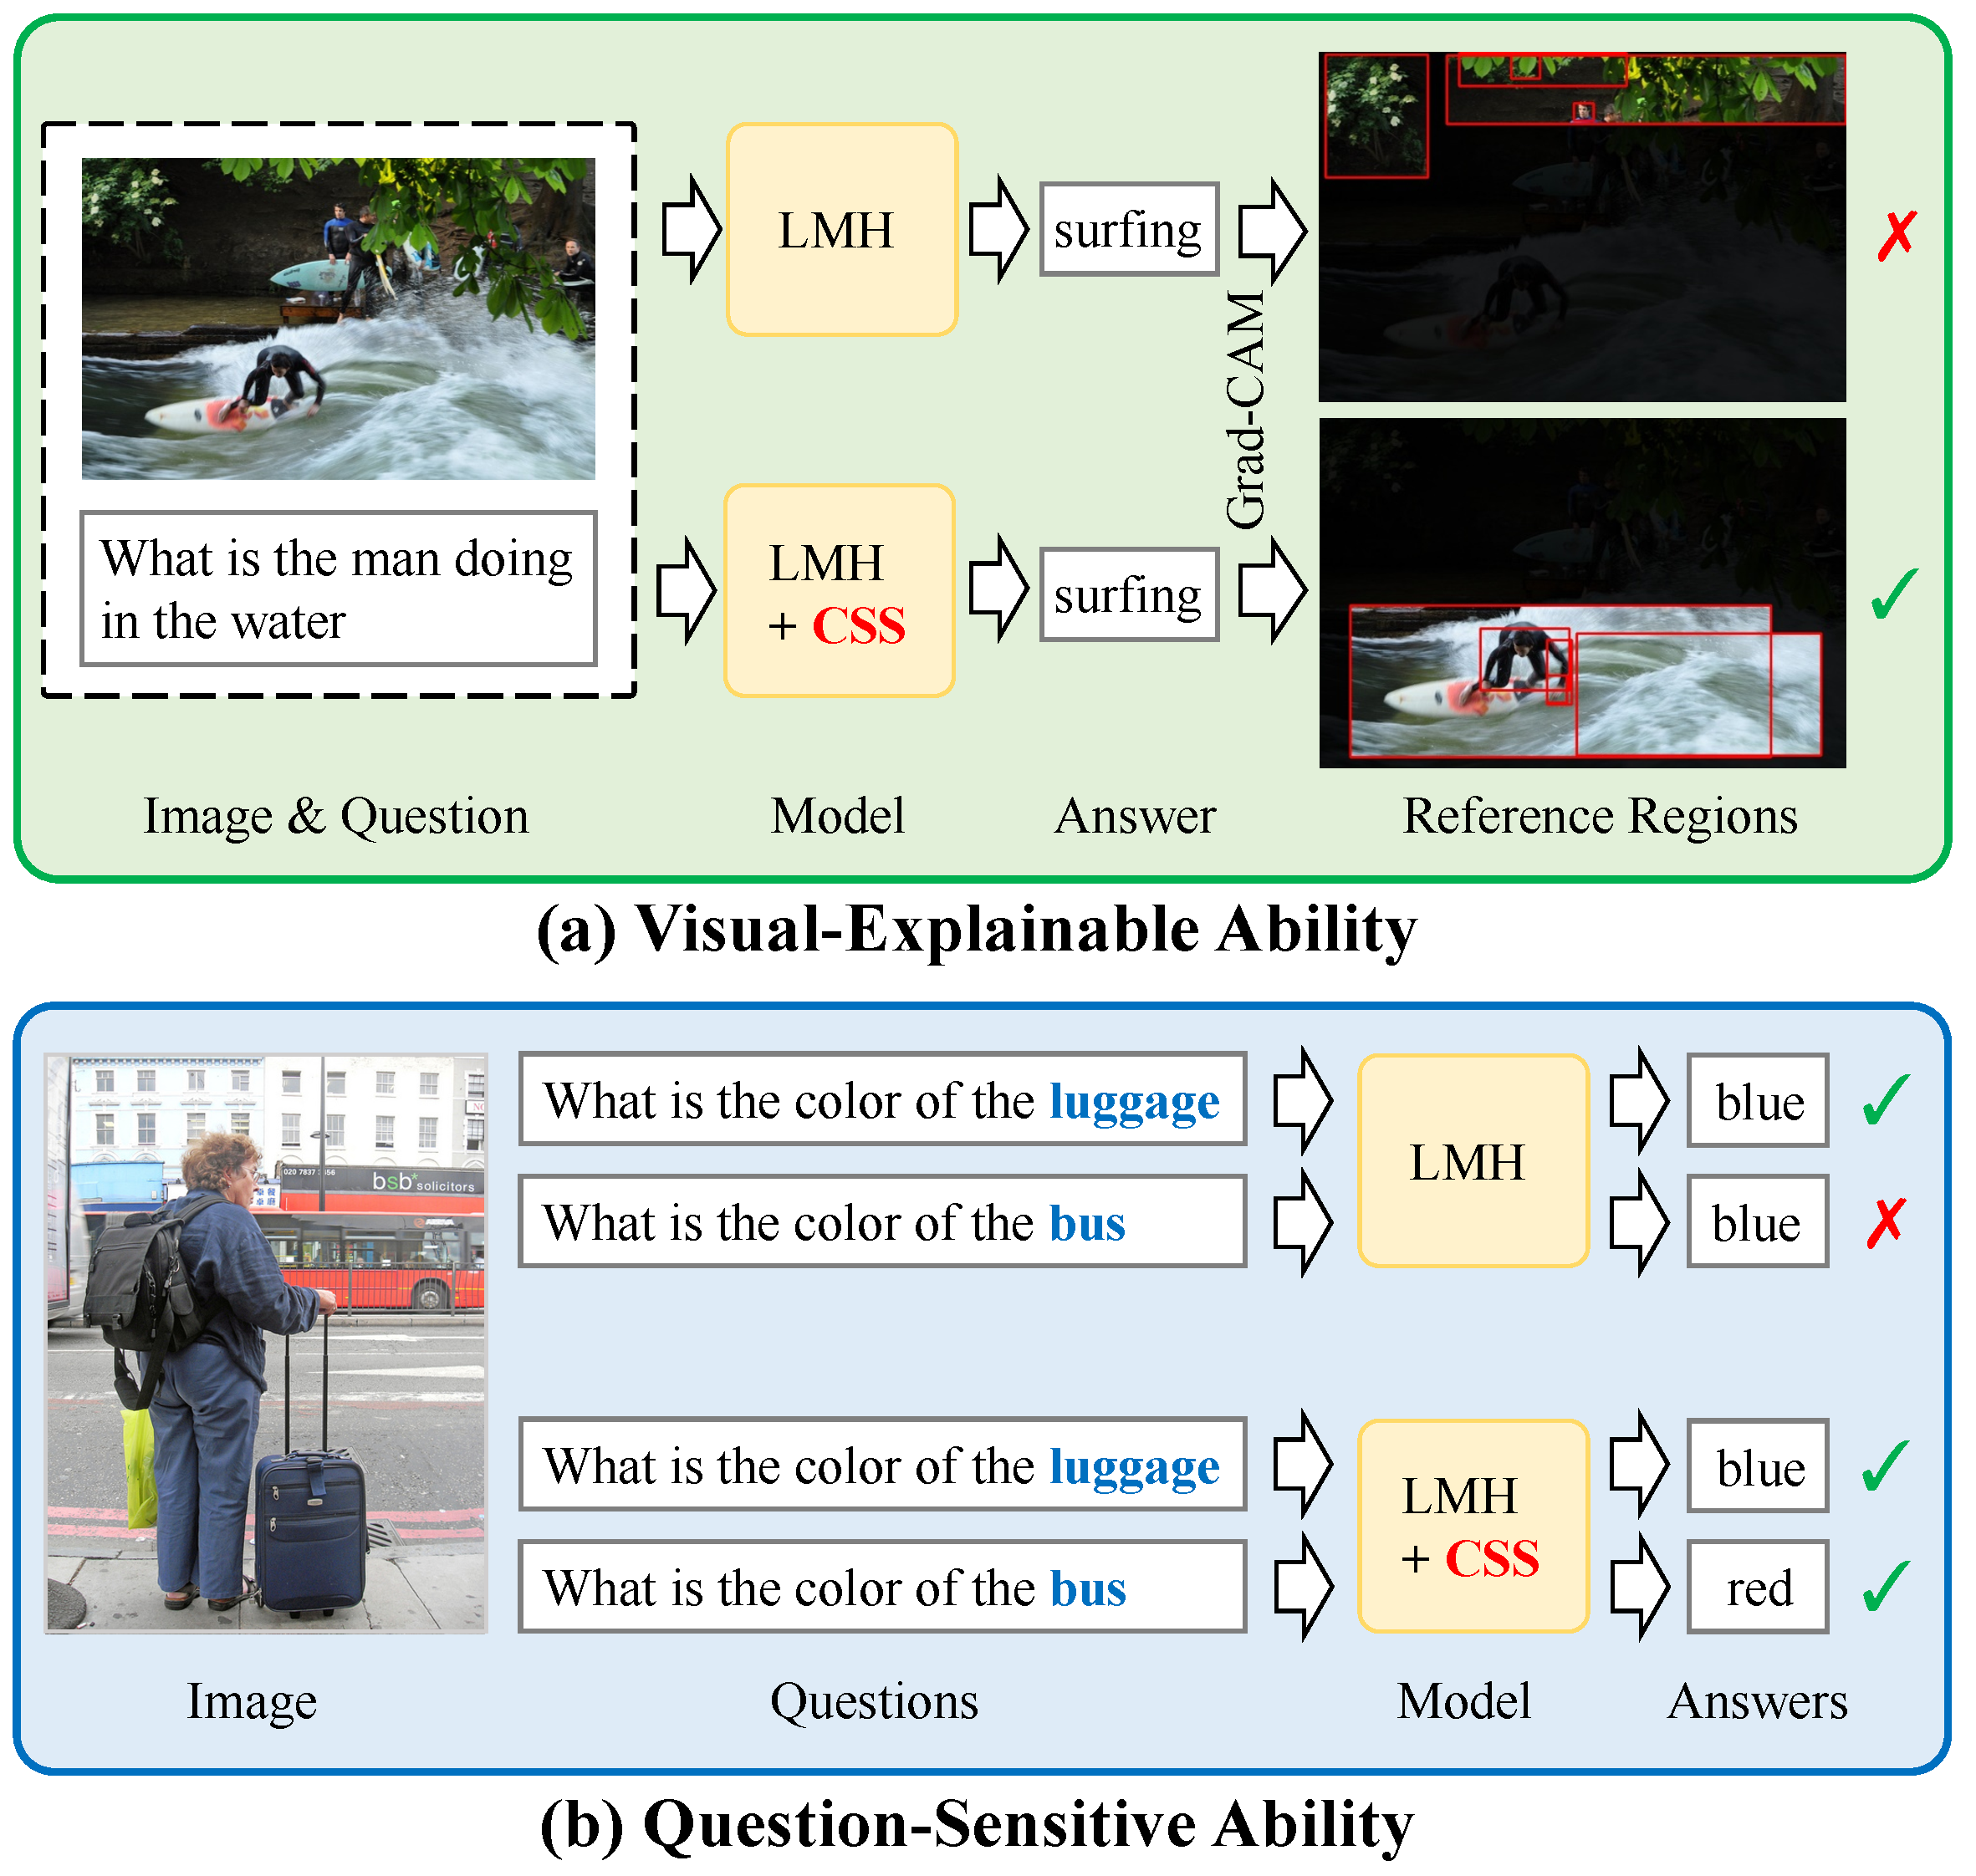
\includegraphics[width=0.85\linewidth]{chapter7/res/motivation.pdf}
    \caption{VQA模型的视觉可解释性和问题敏感性}
    \label{ch7:fig:motivation}
\end{figure}

目前,对于数据集VQA-CP,性能最好的模型是基于复合模型的框架:这些模型通过引入一个辅助网络来约束目标视觉问答网络的训练,其中辅助网络只使用问题作为输入信号。具体来说,这些复合模型可以细分为两小类:(1)基于对抗学习的方法~\cite{ramakrishnan2018overcoming,grand2019adversarial,belinkov2019don}:它们使用对抗学习~\cite{goodfellow2014generative}的方式来训练这两个网络(视觉问答网络和辅助网络),即减少视觉问答网络的损失函数,同时增大辅助网络的损失函数。因为这两个网络共享了同一个文本编码器,所以这类基于对抗学习的方法本质上希望通过学习到一个不含文本偏置的问题编码向量来缓解模型过于依赖文本偏置的问题。然而,Grand等人~\cite{grand2019adversarial}通过实验表明,这类基于对抗学习的方法在计算梯度过程中引入大量噪声,容易造成训练过程的不稳定。(2)基于融合的方法~\cite{cadene2019rubi,clark2019don,mahabadi2019simple}:它们将两个网络预测的答案概率分布进行融合,然后根据融合后的概率分布来计算参数优化的梯度。这类方法的设计动机是让视觉问答模型更加关注一些辅助网络无法回答的训练样本。

\begin{figure}[t]
    \centering
        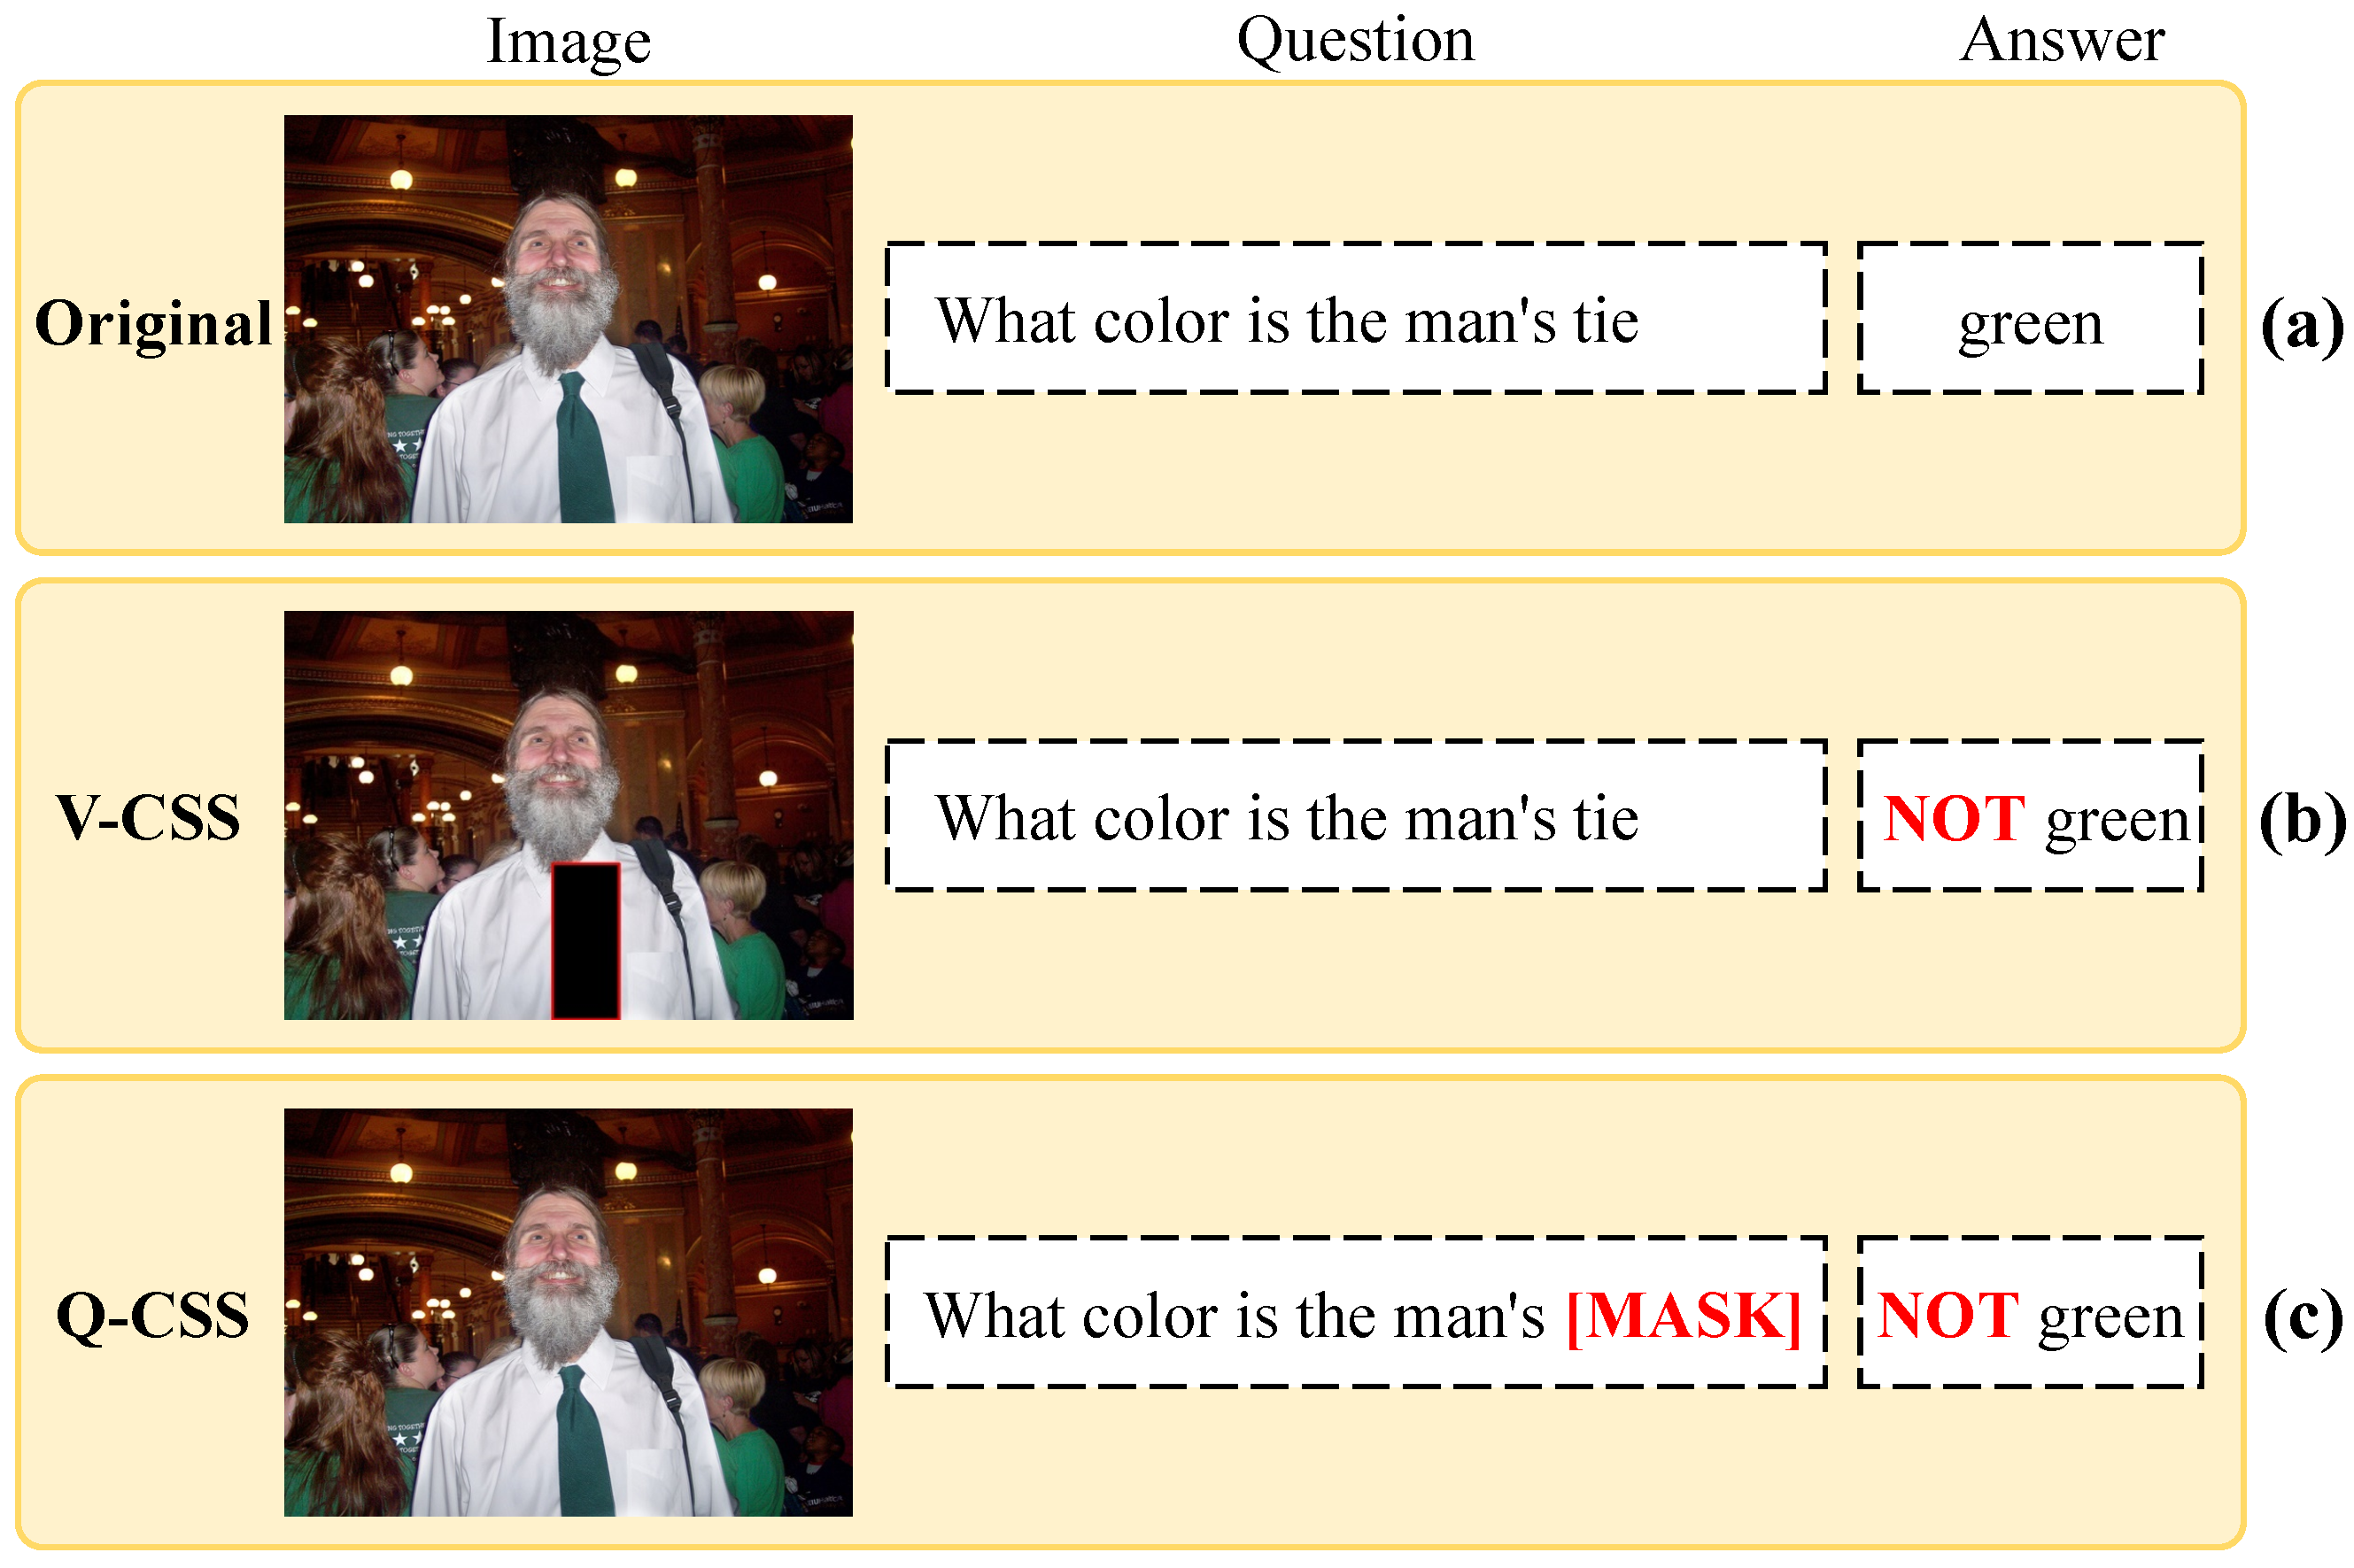
\includegraphics[width=0.85\linewidth]{chapter7/res/V-CSS_Q-CSS.pdf}
    \caption{CSS机制中V-CSS和Q-CSS示例图}
    \label{ch7:fig:V-CSS_Q-CSS}
\end{figure}

尽管这些复合模型在数据集VQA-CP上取得了最佳的实验性能,但是由于目前复合模型这些复杂的网络设计,使得这类模型难以满足一个理想视觉问答模型应该具体的两个特性:(1)\textbf{视觉可解释性}:在预测答案时,模型应该关注正确的视觉图像区域~\cite{ross2017right}。如图~\ref{ch7:fig:motivation}(a)所示,尽管两个模型(LMH和LMH-CSS)都可以预测出正确的答案“surfing”,但实际上这两个模型在做决策时是依据完全不同的视觉区域。(2)\textbf{问题敏感性}:当改变问题时,模型应该能够感知问题的变化,并相应地调整预测结果。如图~\ref{ch7:fig:motivation}(b)所示,当两个问题的句式结构十分接近时(如只替换问题对象“luggage”为“bus”),当两个问题的意思已经完全不同时,模型应该能够感知这两个问题的差异,并将预测从“blue”变成“red”。

在本章,我们提出了一个全新的反事实样本生成机制(CSS),来提升视觉问答模型的视觉可解释性和问题敏感性。如图~\ref{ch7:fig:V-CSS_Q-CSS}所示,CSS机制包含两种不同的样本生成方法:V-CSS和Q-CSS。对于V-CSS而言,我们通过遮盖图像中的重要区域,得到反事实图像。这些“重要区域”是指针对回答该问题时模型需要依据或者关注的图像区域。生成的反事实图像和原始问题就组成了一个新的图像问题对。对于Q-CSS而言,我们通过将原始问题中的重要单词替换成一个特定的词“[MASK]”,得到反事实问题。同样,生成的反事实问题和原始图像也组成了一个新的图像问题对。除了图像问题对,一个标准的视觉问答训练样本还需要相应的标准答案。为了避免大量的人工标注,我们设计了一个动态的答案生成机制,对新合成的图像问题对分配合理的“标准”答案(如:图~\ref{ch7:fig:V-CSS_Q-CSS}中的“not green”)。最后,通过使用原始训练样本和新生成的训练样本一起对视觉问答模型进行训练,迫使模型更加关注被遮盖的重要区域和重要单词。

我们在VQA-CP数据集上通过大量的定性和定量实验都验证了CSS机制的有效性。CSS机制可以无缝地运用在任何视觉问答模型中,包括复合模型。它不仅可以提升模型的视觉可解释性和问题敏感性,同时可以进一步提升模型在VQA-CP上的准确率。值得注意的是,当对视觉问答模型LMH~\cite{clark2019don}使用CSS机制后,模型在数据集VQA-CP v2上可以达到58.95\%的准确率。


\section{反事实样本生成}

对于视觉问答任务,我们将其看成一个多类别分类任务。为了不失一般性,给定一个视觉问答数据集$\mathcal{D} = \{I_i, Q_i, a_i \}^N_i$包含大量的图像$I_i \in \mathcal{I}$、问题$Q_i \in \mathcal{Q}$和答案$a_i \in \mathcal{A}$,视觉问答任务需要学习一个映射函数$f_{vqa}: \mathcal{I} \times \mathcal{Q} \rightarrow [0, 1]^{|\mathcal{A}|}$,可以对任意的图像问题对预测一个答案概率分布。为了后续表达的简洁性,我们在表述中省略了下角标$i$。

在本节,我们先介绍视觉问答中的自底向上和自顶向下模型~\cite{anderson2018bottom},以及复合模型。然后,我们再介绍CSS机制的具体细节。

\subsection{引言}

\textbf{\kaishu{自底向上和自顶向下模型}}(Bottom-Up Top-Down, UpDn):对于每张图像$I$,UpDn模型使用图像编码器$e_v$将图像编码成一系列物体特征:$\bm{V} = \{\bm{v}_1, ..., \bm{v}_{n_v}\}$,其中$\bm{v}_i$表示第$i$个物体特征。对于每个问题$Q$,UpDn模型使用问题编码器$e_q$编码成一系列单词特征:$\bm{Q} = \{\bm{w}_1, ..., \bm{w}_{n_q}\}$,其中$\bm{w}_j$表示第$j$个单词的特征。然后将特征$\bm{V}$和$\bm{Q}$同时输入到模型$f_{vqa}$中来预测答案的概率分布:
\begin{equation} \label{ch7:eq:p_vqa}
    P_{vqa}(\bm{a}|I, Q) = f_{vqa}(\bm{V}, \bm{Q}),
\end{equation}
其中,模型$f_{vqa}$通常包含一个注意力机制,然后利用答案分类的交叉熵作为损失函数对模型进行优化。

\textbf{\kaishu{复合模型}}:根据前文(第~\ref{ch7:sec:introduction}节)讨论,复合模型可以细分为两小类:基于对抗学习的方法和基于融合的方法。因为基于对抗学习的方法~\cite{ramakrishnan2018overcoming,grand2019adversarial,belinkov2019don}训练过程不稳定同时性能相对较低。在本节,我们只介绍基于融合的方法~\cite{cadene2019rubi,clark2019don,mahabadi2019simple}。具体如算法~\ref{ch7:alg:VQA}所示,它们通过引入一个辅助网络$f_q$,其中$f_q$只使用问题$\bm{Q}$做为输入直接预测答案概率:
\begin{equation}
P_{q}(\bm{a}|Q) = f_{q}(\bm{Q}),
\end{equation}
然后,它们通过一个融合函数$M$将两个网络预测的答案概率分布进行融合,得到:
\begin{equation}
\hat{P}_{vqa}(\bm{a}|I, Q) = M(P_{vqa}(\bm{a}|I, Q), P_{q}(\bm{a}|Q)).
\end{equation}
在训练阶段,它们根据融合后的答案概率分布$\hat{P}_{vqa}(\bm{a})$来计算交叉熵损失,进而计算梯度并同时优化网络$f_{vqa}$和网络$f_q$。在测试阶段,它们只使用网络$f_{vqa}$的预测结果作为最终结果。

\begin{algorithm}[t]
    \caption{复合模型(基于融合的方法)}\label{ch7:alg:VQA}
    \begin{algorithmic}[1]
        \Function {$\mathcal{VQA}$}{$I, Q, a, cond$}
        \State $ \bm{V} \leftarrow e_v(I) $
        \State $ \bm{Q} \leftarrow e_q(Q) $
        \State $ P_{vqa}(\bm{a}) \leftarrow f_{vqa}(\bm{V}, \bm{Q}) $
        \State $ P_{q}(\bm{a}) \leftarrow f_{q}(\bm{Q})$      \Comment{辅助模型}
        \State $ \hat{P}_{vqa}(\bm{a}) \leftarrow M(P_{vqa}(\bm{a}), P_{q}(\bm{a}))  $
        \State $ Loss \leftarrow \text{XE}(\hat{P}_{vqa}(\bm{a}), a)$ \Comment{参数更新}
        \If{$cond$}
        \State \textbf{return} $\bm{V}, \bm{Q}, P_{vqa}(\bm{a})$
        \EndIf 
        \EndFunction
    \end{algorithmic}
\end{algorithm}

\subsection{反事实样本生成} 
整个反事实样本生成机制(CSS)的流程展示在算法~\ref{ch7:alg:CSS}上。具体来说,对于给定的一个视觉问答模型(即$\mathcal{VQA}$)和训练样本$(I, Q, a)$,CSS机制主要包含三个步骤:

1. 用原始的训练样本对$\mathcal{VQA}$模型进行训练;

2. 用V-CSS生成反事实样本$(I^-, Q, a^-)$或用Q-CSS生成反事实样本$(I, Q^-, a^-)$;

3. 用新生成的反事实样本对$\mathcal{VQA}$模型进行训练。

在接下来,我们先详细介绍两种反事实样本生成方式:V-CSS和Q-CSS。如算法~\ref{ch7:alg:CSS}所示,对于每个训练样本,我们只使用特定的一种样本生成机制,其中$\delta$是一个超参数来权衡两种生成方式的比例。


\begin{algorithm}[t]
    \caption{反事实样本生成}\label{ch7:alg:CSS}
    \begin{algorithmic}[1]
        \Function {$\mathcal{CSS}$}{$I, Q, a$}
        \State $ \bm{V}, \bm{Q}, P_{vqa}(\bm{a}) \leftarrow \mathcal{VQA}(I, Q, a, \text{True})$
        \State $ cond \sim U[0, 1]$
        \If {$cond \geq \delta $}  \Comment{执行V-CSS}
            \State $ \mathcal{I} \leftarrow  \textsc{IO\_Sel}(I, Q) $
            \State $ s(a, \bm{v}_i) \leftarrow \mathcal{S}(P_{vqa}(a), \bm{v}_i)$
            \State $ I^+, I^- \leftarrow \textsc{CO\_Sel}(\mathcal{I}, \{s(a, \bm{v}_i) \}) $
            \State $ a^- \leftarrow \textsc{DA\_Ass}(I^+, Q, \mathcal{VQA}, a) $
            \State $ \mathcal{VQA}(I^-, Q, a^-, \text{False})$
        \Else \Comment{执行Q-CSS}
            \State $ s(a, \bm{w}_i) \leftarrow \mathcal{S}(P_{vqa}(a), \bm{w}_i) $
            \State $ Q^+, Q^- \leftarrow \textsc{CW\_Sel}(\{s(a, \bm{w}_i)\})$
            \State $ a^- \leftarrow \textsc{DA\_Ass}(I, Q^+, \mathcal{VQA}, a) $
            \State $ \mathcal{VQA}(I, Q^-, a^-, \text{False})$
        \EndIf
        \EndFunction
    \end{algorithmic}
\end{algorithm}

\textbf{V-CSS}:我们将按照算法~\ref{ch7:alg:CSS}中程序执行的顺序依次介绍V-CSS中的主要步骤,包括初始物体选择(\textsc{IO\_Sel})、物体局部贡献计算、重要物体选择(\textsc{CO\_Sel})和动态答案生成(\textsc{DA\_Ass}):

(1)初始物体选择(\textsc{IO\_Sel}):对于任意一个图像问题对$(Q, a)$,通常只有图像中部分物体与当前问题有关。为了缩小重要物体的选择范围,我们首先构建一个小的物体集$\mathcal{I}$,使得$\mathcal{I}$中的物体都可能与当前问题有关。由于数据集中缺乏人工的标注信息,我们参考Wu等人~\cite{wu2019self},认为问题和答案中出现的名词往往可能与当前问题有关。具体来说,我们先用spaCy POS tagger~\cite{honnibal2017spacy}提取出问题和答案中的所有名词,然后利用这些名词的GloVe编码~\cite{pennington2014glove}与图像中所有物体对应类别的GloVe编码计算余弦相似度,其中相似度记为$\mathcal{SIM}$。我们根据相似度$\mathcal{SIM}$直接选择分数最高的$|\mathcal{I}|$个物体组成物体集合$\mathcal{I}$。

(2)物体局部贡献计算:当得到物体集$\mathcal{I}$之后,我们开始计算每个物体对最终的正确答案的贡献。我们参考现有的工作~\cite{jain2019attention,selvaraju2019taking,wu2019self},同样使用修改版的Grad-CAM~\cite{selvaraju2017grad}算法来计算每个物体的局部贡献。对于第$i$个物体来说,它对正确答案$a$的局部贡献为:
\begin{equation} \label{ch7:eq:eq_4}
s(a, \bm{v}_i) = \mathcal{S}(P_{vqa}(a), \bm{v}_i) \coloneqq (\nabla_{\bm{v}_i} P_{vqa}(a))^T\mathbf{1},
\end{equation}
其中$P_{vqa}(a)$是正确答案$a$的预测概率,$\bm{v}_i$是第$i$个物体特征,$\mathbf{1}$是所有元素都为1的向量。显然,当分数$s(a, \bm{v}_i)$越高时,物体特征$\bm{v}_i$对正确答案$a$的贡献也越大。

\begin{algorithm}[t]
    \caption{动态答案生成}\label{ch7:alg:daass}
    \begin{algorithmic}[1]
        \Function {$\textsc{DA\_Ass}$}{$I^+, Q^+, \mathcal{VQA}, a$}
        \State  $\mathcal{VQA}$.eval() \Comment{不更新参数}
        \State  $ \_, \_, P_{vqa}^+(\bm{a}) \leftarrow \mathcal{VQA}(I^+, Q^+, a, \text{True}) $
        \State $ a^+ \leftarrow \text{top-N}(\text{argsort}_{a_i \in \mathcal{A}}(P_{vqa}^+(a_i)))$
        \State $ a^- \coloneqq \{a_i | a_i \in a, a_i \notin a^+ \} $ \Comment{$a$是标准答案集}
        \State \textbf{return} $a^-$
        \EndFunction
    \end{algorithmic}
\end{algorithm}

(3)重要物体选择(\textsc{CO\_Sel}):在对物体集$\mathcal{I}$中所有物体都计算局部贡献$s(a, \bm{v}_i)$之后,我们将分数最高的前K个物体当成重要的物体,记为集合$I^+$。对于每张图像,K是满足公式~\eqref{ch7:eq:eq_5}的最小整数:
\begin{equation} \label{ch7:eq:eq_5}
\sum_{\bm{v}_i \in I^+} \exp(s(a, \bm{v}_i)) / \sum_{\bm{v}_j \in \mathcal{I}} \exp(s(a, \bm{v}_j))  > \eta,
\end{equation}
其中$\eta$是一个超参数用于控制K的数量。在所有的实验中,我们将$\eta$设为0.65。然后,反事实图像就是物体集合$I^+$在所有物体集合$I$中的补集,即$I^- = I \backslash I^+$。如图~\ref{ch7:fig:IQ+-}所示,$I^+$和$I^-$是两个互补的两个物体集合,同时满足$I^+ \cup I^- = I$。

(4)动态答案生成(\textsc{DA\_Ass}):给定反事实图像$I^-$和原始问题$Q$,我们可以组成一个新的图像问题对($I^-, Q$)。作为一个视觉问答任务的训练样本,新的图像问题对同样需要分配“标准”答案。为了减少大量的人工标注,我们设计了一种动态的答案生成机制,来预测标准答案$a^-$。动态答案生成机制的细节在算法~\ref{ch7:alg:daass}中。具体来说,我们将另一个图像问题对($I^+, Q$)输入到视觉问答模型$\mathcal{VQA}$中,然后得到预测的答案概率分布$P^+_{vqa}(\bm{a})$。根据概率$P^+_{vqa}(\bm{a})$,我们选取前N个答案作为$a^+$,然后定义$ a^- \coloneqq \{a_i | a_i \in a, a_i \notin a^+ \}$。它的设计理念就是,图像问题对($I^-, Q$)的标准答案是($I^+, Q$)遗漏的答案。在极端情况下,如果模型对于图像问题对($I^+, Q$)可以预测全部的正确答案,即$a \subset a^+$,则$a^-$为空集$\emptyset$。

\begin{figure}[t]
    \centering
        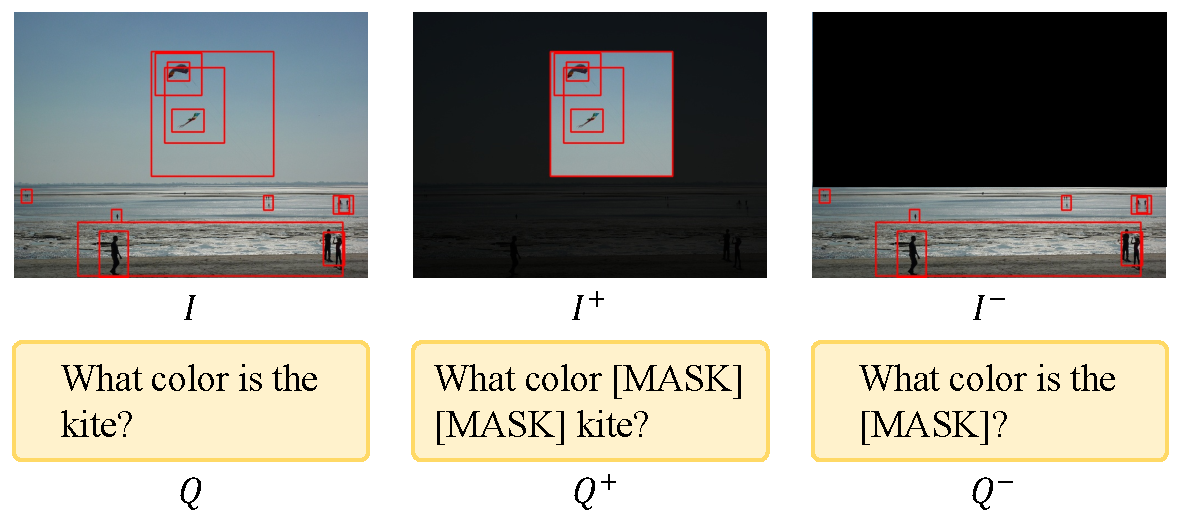
\includegraphics[width=0.9\linewidth]{chapter7/res/IQ+-.pdf}
    \caption{CSS机制中一个$I^+$、$I^-$、$Q^+$和$Q^-$的示例图}
    \label{ch7:fig:IQ+-}
\end{figure}

\textbf{Q-CSS}:Q-CSS方式的主要步骤和V-CSS方式非常接近,除了没有初始物体选择(即\textsc{IO\_Sel})。按照算法~\ref{ch7:alg:CSS}的执行顺序,Q-CSS主要包含三步:单词局部贡献计算、重要单词选择(\textsc{CW\_Sel})和动态答案生成(\textsc{DA\_Ass}):

(1)单词局部贡献计算:与V-CSS中物体局部贡献计算相似(公式~\eqref{ch7:eq:eq_4}),对于第$i$个单词,它对正确答案$a$的贡献为:
\begin{equation} \label{ch7:eq:eq_6}
s(a, \bm{w}_i) = \mathcal{S}(P_{vqa}(a), \bm{w}_i) \coloneqq (\nabla_{\bm{w}_i} P_{vqa}(a))^T\mathbf{1}.
\end{equation}

(2)重要单词选择(\textsc{CW\_Sel}):对于这步,我们首先提取每个问题$Q$的问题类别前缀,这些前缀直接使用数据集VQA-CP中默认的问题类别前缀。然后对剩余的单词选择贡献最高的K个单词作为重要单词,而反事实问句$Q^-$就是将问句$Q$中的重要单词替换成一个特殊字符“[MASK]”。如图~\ref{ch7:fig:IQ+-},当问句是“what color is the kite”以及重要单词是“kite”时,反事实问句$Q^-$为“what color is the [MASK]”,而$Q^+$为“what color [MASK] [MASK] kite”。

(3)动态答案生成(\textsc{DA\_Ass}):这个动态答案生成步骤和V-CSS的完全相同,即算法~\ref{ch7:alg:daass}。与V-CSS唯一不同的是,对于Q-CSS,\textsc{DA\_Ass}的输入是图像问题对$(I, Q^+)$,而V-CSS的输入是图像问题对$(I^+, Q)$。


\section{实验设置与性能对比}

我们主要在数据集VQA-CP~\cite{agrawal2018don}的测试集上对模型的性能进行验证。为了实验比较的完整性,我们同样在数据集VQA v2~\cite{goyal2017making}的验证集上进行测试。关于模型的准确率,我们使用通用的VQA准确率计算方式~\cite{antol2015vqa}。为了实验比较的公平性,所有的实验都采取与UpDn模型~\cite{anderson2018bottom}相同的数据预处理。

\subsection{CSS对视觉问答的性能分析}

\textbf{\kaishu{CSS机制中不同超参数对模型性能的影响}}:我们通过大量的对比实验来分析V-CSS和Q-CSS中不同超参数对模型性能的影响。具体来说,所有的实验都是基于现有的视觉问答模型LMH~\cite{clark2019don}。实验结果展示在图~\ref{ch7:fig:ablative_studies}中。

(1)V-CSS中初始物体集$\mathcal{I}$的大小:不同$|\mathcal{I}|$对模型性能的影响如图~\ref{ch7:fig:ablative_studies}(a)所示。随着初始物体集大小$|\mathcal{I}|$的增加,模型的性能逐渐降低。

(2)V-CSS中重要物体选择的数量:不同重要物体选择的数量对实验性能的影响如图~\ref{ch7:fig:ablative_studies}(a)所示。我们比较了动态选择K(公式~\ref{ch7:eq:eq_5})和预先固定一些常数(如:1、3或5)。从实验结果可知,动态选择K个重要物体可以得到最佳的实验性能。

(3)Q-CSS中重要单词选择的数量:不同重要单词的选择数量对实验性能的影响如图~\ref{ch7:fig:ablative_studies}(b)所示。从实验结果可知,只选择1个单词作为重要单词性能最佳。

(4)V-CSS和Q-CSS的比例$\delta$:不同$\delta$对实验性能的影响如图~\ref{ch7:fig:ablative_studies}(c)所示。从实验结果可知,$\delta = 0.5$时性能最佳。

\begin{figure*}[t]
    \centering
    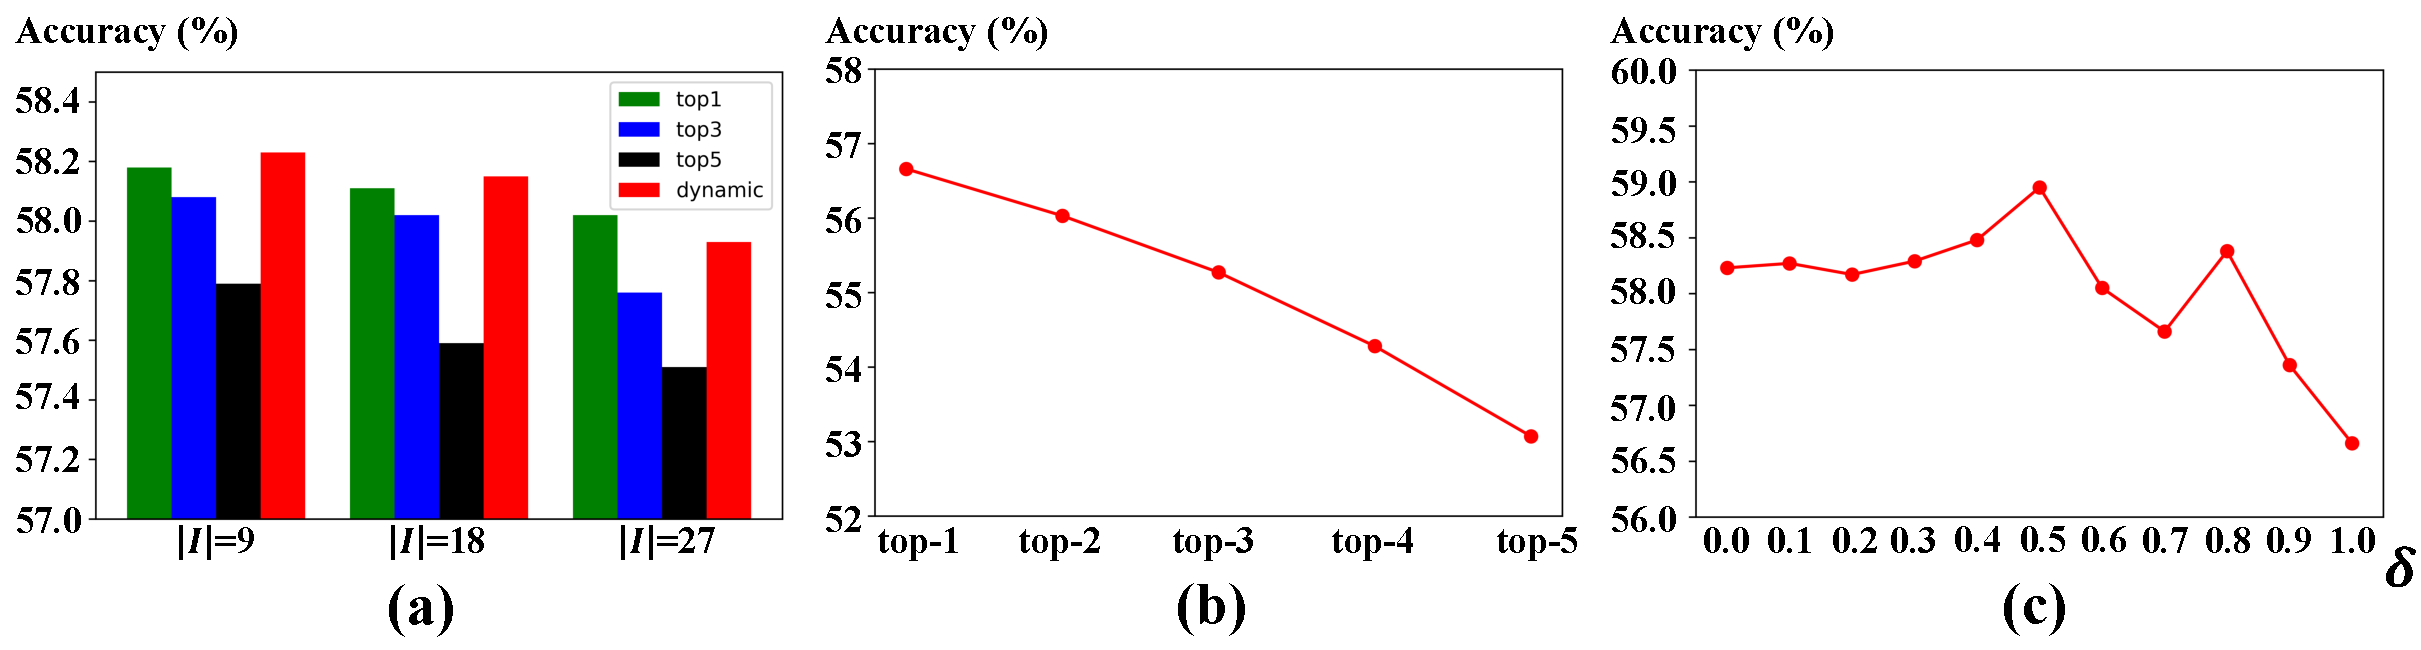
\includegraphics[width=\linewidth]{chapter7/res/ablative_studies.pdf}
    \caption{V-CSS和Q-CSS中不同超参数对模型性能的影响}
    \label{ch7:fig:ablative_studies}
\end{figure*}


\textbf{\kaishu{CSS机制对模型的通用性}}:由于CSS机制的设计没有依赖任何具体的VQA模型设计,为了验证CSS机制对不同模型结构的通用性,我们将CSS机制应用于多种VQA模型中:\textbf{UpDn}~\cite{anderson2018bottom}、\textbf{PoE} (Product of Experts)~\cite{clark2019don,mahabadi2019simple}、\textbf{RUBi}~\cite{cadene2019rubi}和\textbf{LMH}~\cite{clark2019don}。其中模型PoE、RUBi、LMH都属于复合模型。所有的实验结果展示在表~\ref{ch7:tab:boost_models}中,$^\dagger$表示实验结果为我们自己的重现结果。

由表~\ref{ch7:tab:boost_models}中结果可以看出,CSS机制可以提升多种不同的视觉问答模型的性能。尤其对于复合模型来说,性能的提升往往更加明显(例如:在模型LMH和模型PoE中准确率可以分别提升6.5\%和9.79\%)。在通常情况下,相比于单独使用一种CSS机制(V-CSS或Q-CSS),同时使用两种CSS机制(即$\mathcal{CSS}$)可以得到最佳性能。

%%%%%% Boost Ensemble-based Models  %%%%%%%%%%%%%%%
\begin{table}[tbp]
    \begin{center}
        \scalebox{0.90}{
            \begin{tabular}{|l | l | l | c c c c|}
                \hline
                & & Model & All & Y/N & Num & Other  \\
                \hline
                \parbox[t]{2mm}{\multirow{5}{*}{\rotatebox[origin=c]{90}{Plain Models}}} & \multirow{5}{*}{UpDn~\cite{anderson2018bottom}} & Baseline & 39.74 & 42.27 & 11.93  & 46.05 \\
                & & Baseline$^\dagger$ & 39.68 & 41.93 & 12.68 & 45.91 \\
                & & ~~~~~~~~+Q-CSS & 40.05 & 42.16 & 12.30 & 46.56 \\
                & & ~~~~~~~~+V-CSS & 40.98 & 43.12 & 12.28 & 46.86 \\
                & & ~~~~~~~~+$\mathcal{CSS}$ & \textbf{41.16} & \textbf{43.96} & \textbf{12.78} & \textbf{47.48} \\
                \hline
                \parbox[t]{2mm}{\multirow{15}{*}{\rotatebox[origin=c]{90}{Ensemble-Based Models}}} & \multirow{5}{*}{PoE~\cite{clark2019don, mahabadi2019simple}} & Baseline & 39.93 & -- & --  & -- \\
                & & Baseline$^\dagger$ & 39.86 & 41.96 & 12.59 & 46.25 \\
                & & ~~~~~~~~+Q-CSS & 40.73 & 42.99 & 12.49 & \textbf{47.28} \\
                & & ~~~~~~~~+V-CSS & \textbf{49.65} & \textbf{74.98} & \textbf{16.41} & 45.50 \\
                & & ~~~~~~~~+$\mathcal{CSS}$& 48.32 & 70.44 & 13.84 & 46.20 \\
                \cline{2-7}
                & \multirow{5}{*}{RUBi~\cite{cadene2019rubi}} & Baseline & 44.23 & -- & --  & -- \\
                & & Baseline$^\dagger$ & 45.23 & 64.85 & 11.83 & 44.11 \\
                & & ~~~~~~~~+Q-CSS & 46.31 & \textbf{68.70} & \textbf{12.15} & 43.95 \\
                & & ~~~~~~~~+V-CSS & 46.00 & 62.08 & 11.84 & \textbf{46.95} \\
                & & ~~~~~~~~+$\mathcal{CSS}$ & \textbf{46.67} & 67.26 & 11.62 & 45.13 \\
                \cline{2-7}
                & \multirow{5}{*}{LMH~\cite{clark2019don}} & Baseline & 52.05 & -- & --  & -- \\
                & & Baseline$^\dagger$ & 52.45 & 69.81 & 44.46 & 45.54 \\
                & & ~~~~~~~~+Q-CSS & 56.66 & 80.82 & 45.83 & 46.98 \\
                & & ~~~~~~~~+V-CSS & 58.23 & 80.53 & \textbf{52.48} & 48.13 \\
                & & ~~~~~~~~+$\mathcal{CSS}$ & \textbf{58.95} & \textbf{84.37} & 49.42 & \textbf{48.21} \\
                \hline
            \end{tabular}
        } % scale box
    \end{center}
    \caption{CSS机制对不同VQA模型的性能影响}
    \label{ch7:tab:boost_models}
\end{table}

\subsection{视觉问题方法性能对比}

\textbf{\kaishu{数据集VQA-CP v2和VQA v2上性能对比}}:
我们将CSS机制应用于模型LMH~\cite{clark2019don}中,然后将模型标记为模型\textbf{LMH-CSS}。我们将模型LMH-CSS与其他目前性能最好的视觉问答模型在数据集VQA-CP v2和VQA v2上进行性能对比。根据模型的骨干网络不同,我们可以将模型分为两大类:(1)\textbf{AReg}~\cite{ramakrishnan2018overcoming}、\textbf{MuRel}~\cite{cadene2019murel}、\textbf{GRL}~\cite{grand2019adversarial}、\textbf{RUBi}~\cite{cadene2019rubi}、\textbf{SCR}~\cite{wu2019self}、\textbf{LMH}~\cite{clark2019don}和\textbf{HINT}~\cite{selvaraju2019taking}。这些模型都是将模型\textbf{UpDn}~\cite{anderson2018bottom}作为骨干网络。(2)\textbf{HAN}~\cite{malinowski2018learning}、\textbf{GVQA}~\cite{agrawal2018don}、\textbf{ReGAT}~\cite{li2019relation}、\textbf{NSM}~\cite{hudson2019learning}。这些模型都是使用其他不同的骨干网络。例如:模型\textbf{BLOCK}~\cite{ben2019block}、模型\textbf{BAN}~\cite{kim2018bilinear} 等。特别地,模型AReg、GRL、RUBi和LMH都是复合模型。

实验结果都展示在表~\ref{ch7:tab:SOTA_v2}中。当在数据集VQA-CP v2上进行训练和测试时,模型LMH-CSS在所有的问题类别上都可以达到当时最好实验性能。特别地,CSS机制可以大幅提升模型LMH6.5\%的准确率(58.95\%相比于52.45\%)。当在数据集VQA v2上进行训练和测试时,CSS机制会造成细微的性能下降(1.74\%)。为了评估不同模型对文本偏置的依赖,我们对比了模型在两个不同数据集中性能的差异。相比于之前的模型过于依赖文本偏置(例如:模型UpDn和模型LMH在数据集VQA-CP v2和数据集VQA v2的性能差分别为23.74\%和9.19\%),模型LMH-CSS可以显著地减少模型间的性能差异至0.96\%,说明CSS机制可以显著地缓解模型对文本偏置的依赖。


%%%%%%%%%%%%% STOA on VQA-CP v2 %%%%%%%%%%%%%%%%
\begin{table*}
    \begin{center}
        \scalebox{0.85}{
            \begin{tabular}{| l | c c c c | c c c c| c |}
                \hline
                \multirow{2}{*}{Model}  & \multicolumn{4}{c|}{VQA-CP v2 test $\uparrow$} & \multicolumn{4}{c|}{VQA v2 val $\uparrow$} & Gap$\Delta$$\downarrow$ \\
                & All & Yes/No & Num & Other & All & Yes/No & Num & Other & All \\
                \hline
                HAN~\cite{malinowski2018learning} & 28.65 & 52.25 & 13.79 & 20.33 & -- & -- & -- & -- & --  \\
                GVQA~\cite{agrawal2018don} & 31.30 & 57.99 & 13.68 & 22.14 & 48.24 & 72.03 & 31.17 & 34.65 & 16.94 \\
                ReGAT~\cite{li2019relation} & 40.42 & -- & -- & -- & 67.18 & -- & -- & -- & 26.76 \\
                RUBi~\cite{cadene2019rubi} & 47.11 & 68.65 & 20.28 & 43.18 & 61.16 & -- & -- & -- & 14.05  \\ 
                NSM~\cite{hudson2019learning} & 45.80 & -- & -- & -- & -- & -- & -- & -- & -- \\
                \cline{1-1}
                UpDn~\cite{anderson2018bottom} & 39.74 & 42.27 & 11.93 & 46.05 & 63.48 & 81.18 & 42.14 & 55.66 & 23.74 \\
                ~~~~+AReg$^\dagger$~\cite{ramakrishnan2018overcoming} & 41.17 & 65.49 & 15.48 & 35.48 & 62.75 & 79.84 & 42.35 & 55.16 & 21.58 \\
                ~~~~+MuRel~\cite{cadene2019murel} & 39.54 & 42.85 & 13.17 & 45.04 & -- & -- & -- & --  & -- \\
                ~~~~+GRL$^\dagger$~\cite{grand2019adversarial} & 42.33 & 59.74 & 14.78 & 40.76 & 51.92 & -- & -- & -- & 9.59 \\
                ~~~~+RUBi$^\dagger$$^*$~\cite{cadene2019rubi} & 45.23 & 64.85 & 11.83 & 44.11 & 50.56 & 49.45 & 41.02 & 53.95 & 5.33  \\
                ~~~~+SCR~\cite{wu2019self} & 48.47 & 70.41 & 10.42 & 47.29 & 62.30 & 77.40 & 40.90 & 56.50 & 13.83  \\
                ~~~~+LMH$^\dagger$$^*$~\cite{clark2019don} & 52.45 & 69.81 & 44.46 & 45.54 & 61.64 & 77.85 & 40.03 & 55.04 & 9.19  \\
                ~~~~+\textbf{LMH-CSS} & \textbf{58.95} & \textbf{84.37} & \textbf{49.42} & \textbf{48.21} & 59.91 & 73.25 & 39.77 & 55.11 & \textbf{0.96}  \\
                \hline\hline
                ~~~~+HINT+HAT~\cite{selvaraju2019taking} & 47.70 & 70.04 & 10.68 & 46.31 & 62.35 & 80.49 & 41.75 & 54.01 & 14.65 \\
                ~~~~+SCR+HAT~\cite{wu2019self} & 49.17 & 71.55 & 10.72 & 47.49 & 62.20 & 78.90 & 41.40 & 54.30 & 13.03  \\
                ~~~~+SCR+VQA-X~\cite{wu2019self} & 49.45 & 72.36 & 10.93 & 48.02 & 62.20 & 78.80 & 41.60 & 54.40 & 12.75  \\
                \hline
            \end{tabular}
        } % scale box
    \end{center}
    \caption{不同视觉问答模型在数据集VQA-CP v2和数据集VQA v2上的性能对比} % \footnotemark
    \label{ch7:tab:SOTA_v2}
\end{table*}
%%%%%%%%%%%%%%%%%%%%%%%%%%%%%%%%%%

\textbf{\kaishu{数据集VQA-CP v1上性能对比}}:我们同时将模型LMH-CSS与当时最好的视觉问答模型在数据集VQA-CP v1上进行性能评估。同样,根据骨干网络的不同,我们可以将这些模型分为:(1) \textbf{GVQA}。它是使用模型\textbf{SAN}~\cite{yang2016stacked}模型作为骨干网络。(2)\textbf{AReg}、\textbf{GRL}、\textbf{RUBi}和\textbf{LMH}。这些模型都是使用模型\textbf{UpDn}作为骨干网络。

所有的实验结果都展示在表~\ref{ch7:tab:SOTA_v1}中。通过和其他视觉问答模型对比,模型LMH-CSS在数据集VQA-CP v1上可以达到当时最好的实验性能。特别地,CSS机制可以提升模型LMH5.68\%的准确率(60.95\%相比于55.27\%)。

%%%%%%%%%%%%% STOA on VQA-CP v1 %%%%%%%%%%%%%%%%
\begin{table}[tbp]
    \begin{center}
        \scalebox{0.9}{
            \begin{tabular}{| l | c c c c|}
                \hline
                Model & All & Yes/No & Num & Other  \\
                \hline
                GVQA~\cite{agrawal2018don}  & 39.23 & 64.72 & 11.87 & 24.86 \\
                UpDn~\cite{anderson2018bottom} & 39.74 & 42.27 & 11.93 & \textbf{46.05} \\
                ~~~+AReg$^\dagger$~\cite{ramakrishnan2018overcoming} & 41.17 & 65.49 & 15.48 & 35.48 \\
                ~~~+GRL$^\dagger$~\cite{grand2019adversarial} &  45.69 & 77.64 & 13.21 & 26.97 \\
                ~~~+RUBi$^\dagger$$^*$~\cite{cadene2019rubi} & 50.90 & 80.83 & 13.84 & 36.02 \\
                ~~~+LMH$^\dagger$$^*$~\cite{clark2019don} & 55.27 & 76.47 & 26.66 & 45.68 \\
                \hline
                ~~~+\textbf{LMH-CSS} & \textbf{60.95} & \textbf{85.60} & \textbf{40.57} & 44.62  \\
                \hline
            \end{tabular}
        } % scale box
    \end{center}
    \caption{不同视觉问答模型在数据集VQA-CP v1上的性能对比}
    \label{ch7:tab:SOTA_v1}
\end{table}
%%%%%%%%%%%%%%%%%%%%%%%%%%%%%%%%%


\subsection{CSS机制对视觉可解释性的帮助}

为了验证CSS机制对提升视觉问答模型视觉可解释性的有效性,我们主要回答两个问题:\textbf{Q1}:现有的具备视觉可解释性的模型能否嵌入复合模型的框架?\textbf{Q2}:CSS机制如何提升视觉可解释性的有效性?

\textbf{\kaishu{CSS vs. SCR}}(Q1):我们将当时最好的视觉可解释性模型SCR~\cite{wu2019self}直接嵌入到最好的复合模型LMH中,然后和CSS机制进行对比。实验结果展示在表~\ref{ch7:tab:ablative_q1}中。

因为当时最好的视觉可解释性模型(如:SCR、HINT)都不是端到端直接训练的。为了公平地对比,我们使用一个训练好的LMH模型(VQA-CP v2上达到52.45\%的准确率)作为模型的初始化。然而,实验结果发现,随着模型的训练,模型的性能逐渐降低,这表明这些具备视觉可解释性的模型都不能嵌入到复合模型的框架中。相反,CSS机制可以无缝地嵌入复合模型并进一步提升性能。

\textbf{\kaishu{视觉可解释性评估}}(Q2):我们分别定量和定性地评估CSS机制对提升视觉可解释性的有效性。对于定量结果,由于数据集中缺少人工的标注(即哪些物体为重要物体),我们直接将$\mathcal{SIM}$分数当成人工标注的重要物体。然后我们设计了一个新的评价指标$\mathcal{AI}$(Average Importance):$|s(a, \bm{v})|$分数最高的前K个物体中的平均$\mathcal{SIM}$分数。定量实验结果展示在表~\ref{ch7:tab:ablative_q2}中。对于定性结果,我们将结果展示在图~\ref{ch7:fig:visualization}(a)中。其中绿色框表示分数$s(\hat{a}, \bm{v})$大于0,即对最终预测的答案有正面的贡献的物体;而红色框表示$s(\hat{a}, \bm{v})$小于0,即对最终预测的答案有反面的贡献的物体。只有与问题答案对相关性较大的物体才展示出来(即$\mathcal{SIM}$大于等于0.6)。

%%%%%%%%%%%%% Ablative Studies  %%%%%%%%%%%%%%%
\begin{table}[tbp]
    \begin{center}
    \scalebox{0.9}{
        \begin{tabular}{|l| c c c c|}
            \hline
                Model & All & Yes/No & Num & Other\\
            \hline
                SCR  & 48.47 & 70.41 & 10.42 & 47.29 \\
                LMH &52.45 & 69.81 & 44.46 & 45.54  \\
                LMH+SCR & \multicolumn{4}{c|}{continued decrease} \\
                LMH+$\mathcal{CSS}$ & 58.95 & 84.37 & 49.42 & 48.21 \\
            \hline
        \end{tabular}
    }
    \end{center}
    \caption{数据集VQA-CP v2测试集的准确率}
    \label{ch7:tab:ablative_q1}
\end{table}

\begin{table}[tbp]
    \begin{center}
    \scalebox{0.9}{
        \begin{tabular}{| l | c c c |}
            \hline
                Model & Top-1 & Top-2 & Top-3  \\
            \hline
                UpDn & 22.70 & 21.58 & 20.89 \\
                SCR & 27.58 & 26.29 & 25.38 \\
                LMH & 29.67 & 28.06 & 27.04 \\
                LMH+V-CSS & 30.24 & 28.53 & 27.51 \\
                LMH+$\mathcal{CSS}$& \textbf{33.43} & \textbf{31.27} & \textbf{29.86} \\
            \hline
        \end{tabular}
    }
    \end{center}
    \caption{数据集VQA-CP v2测试集的$\mathcal{AI}$分数}
    \label{ch7:tab:ablative_q2}
\end{table}

\begin{table}[tbp]
    \begin{center}
    \scalebox{0.9}{
        \begin{tabular}{| l |c c c c| c |}
            \hline
                Model & k=1 & k=2 & k=3 & k=4  & $\mathcal{CI}$ \\
            \hline
                UpDn  & 49.94 & 38.80 & 31.55 & 28.08 & 6.01 \\
                LMH & 51.68 & 39.84 & 33.38 & 29.11 & 7.44 \\
                LMH+Q-CSS & 54.83  & 42.34 & 35.48 & 31.02 & 9.02 \\
                LMH+$\mathcal{CSS}$ & \textbf{55.04} & \textbf{42.78} & \textbf{35.63} & \textbf{31.17} & 
                \textbf{9.03} \\
            \hline
        \end{tabular}    
    }
    \end{center}
    \caption{数据集VQA-CP-Rephrasing测试集的$CS(k)$和数据集VQA-CP v2测试集的$\mathcal{CI}$分数}
    \label{ch7:tab:ablative_q3}
\end{table}
%%%%%%%%%%%%%%%%%%%%%%%%%%%%%%%

由表~\ref{ch7:tab:ablative_q2}可以看出,CSS机制可以显著地提升模型的$\mathcal{AI}$分数,即模型做决策时更加依赖与问题答案更加相关的物体。由图~\ref{ch7:fig:visualization}可以看出,CSS机制可以帮助模型提升重要物体的影响(绿色框),抑制不相关物体的影响(红色框)。

\begin{figure}[t]
    \centering
        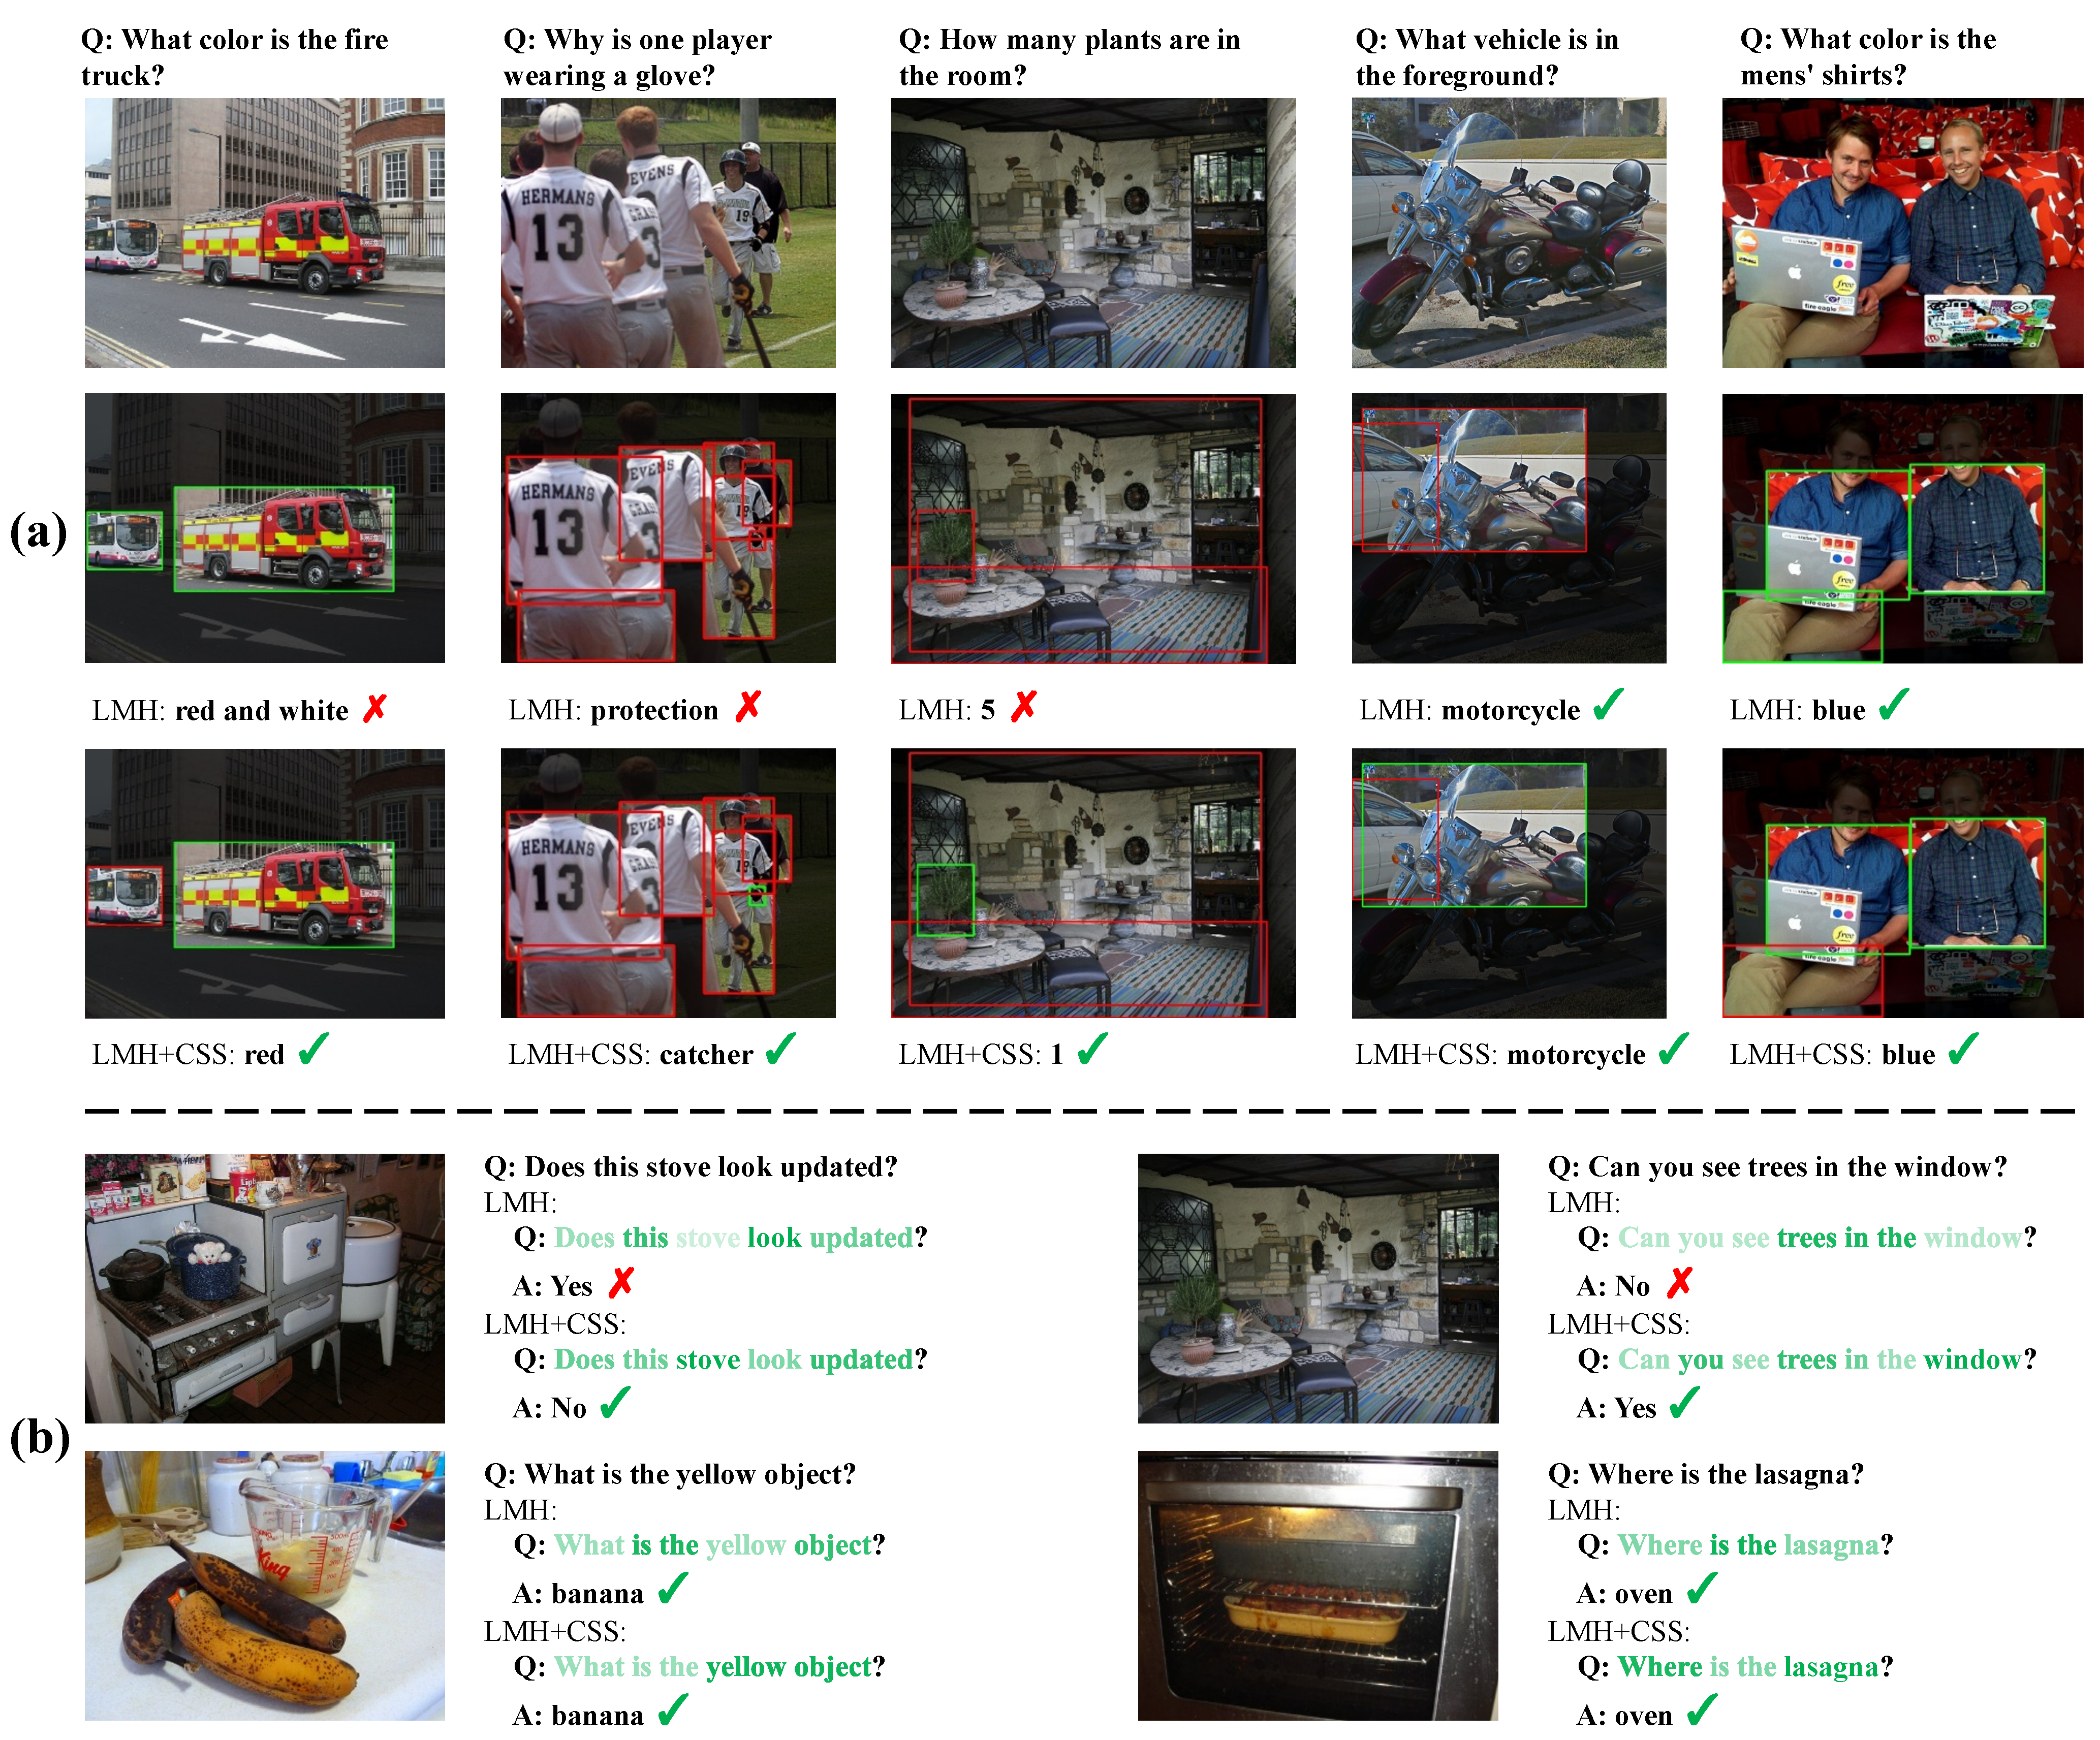
\includegraphics[width=\linewidth]{chapter7/res/visualization.pdf}
    \caption{不同物体和单词对答案预测贡献的可视化结果}
    \label{ch7:fig:visualization}
\end{figure}


\subsection{CSS对问题敏感性的帮助}
为了验证CSS机制对提升视觉问答模型问题敏感性的有效性,我们主要回答两个问题:\textbf{Q3}:CSS机制可以提升模型对不同句式表达的鲁棒性吗?\textbf{Q4} CSS机制如何提升问题敏感性的有效性?

\textbf{\kaishu{对不同句式表达的鲁棒性}}(Q3):根据Shah~\cite{shah2019cycle}等人的讨论,对不同句式表达的鲁棒性是问题敏感性的一种表现。为了准确地评估,我们按照数据集VQA-CP的划分,将现有的数据集VQA-Rephrasings~\cite{shah2019cycle}进行重新划分,记为VQA-CP-Rephrasings。对于评估,我们使用标准评估指标$CS(k)$(Consensus Score)。实验结果展示在表~\ref{ch7:tab:ablative_q3}中。

由表~\ref{ch7:tab:ablative_q3}可以看出,Q-CSS可以显著提升模型对不同句式结果表达的敏感性。当同时使用两种CSS机制时(即$\mathcal{CSS}$),模型可以进一步提升鲁棒性。

\textbf{\kaishu{问题敏感性评估}}(Q4):我们分别在定量和定性地评估CSS机制对提升问题敏感性的有效性。对于定量结果,由于缺少统一的评价指标,我们定义一个新的评价指标$\mathcal{CI}$(Confidence Improvement):给定一个样本$(I, Q, a)$,我们通过去除一个重要单词得到另一个样本$(I, Q^*, a)$,然后将这两个样本同时输入到模型中计算标准答案的置信度下降量。我们定义$\mathcal{CI}$为:
\begin{equation}
\mathcal{CI} = \frac{\sum_{(I, Q)}  (P_{vqa}(a | I, Q) - P_{vqa}(a | I, Q^*)) \cdot \mathbf{1}(a = \hat{a}) }{\sum_{(I, Q)} 1},
\end{equation}
其中$\hat{a}$是模型对样本$(I, Q)$的预测结果,$\mathbf{1}$是指示函数,当$a = \hat{a}$时值为1,否则值为0。所有的结果展示在表~\ref{ch7:tab:ablative_q3}中。对于定性结果,我们将结果展示在图(b)中,其中不同的绿色程度表示$s(\hat{a}, \bm{w})$的相对大小。绿色越深表示该单词对最终模型预测的贡献越大。

由表~\ref{ch7:tab:ablative_q3}可以看出,CSS机制帮助模型在决策时更加依赖与问题答案更加相关的单词,即去除重要单词之后导致更多的置信度下降。从图~\ref{ch7:fig:visualization}中可以发现,CSS机制能够提升模型对问题的理解,更加关注重要的单词,如“stove”、“lasagna”等。


\section{本章小结}
在本章,我们提出了一种全新的反事实样本生成机制(CSS)来提升视觉问答模型的视觉可解释性和问题敏感性,缓解模型对文本偏置的依赖。CSS机制通过遮盖重要的物体和单词,迫使模型更加关注被遮盖的重要区域,同时进一步提升模型预测答案的准确率。因为CSS机制的设计不依赖于任何视觉问答模型,所以CSS机制可以无缝地嵌入任何视觉问答模型中。理论上,CSS机制可以扩展到其他的多模态任务中,缓解文本偏置问题。
